\begin{frame}
\tableofcontents
\end{frame}

%%%%%%%%%%%%%%%%%%%%%%%%
%%%%%%%%%%%%%%%%%%%%%%%%
%%%%%%%%%%%%%%%%%%%%%%%%
%%%%%%%%%%%%%%%%%%%%%%%%

\section{حسگری فشرده\hfill}
%%%%%%%%%%%%%%%%%%%%%%%%
\begin{frame}
\frametitle{حسگری فشرده}

\begin{columns} 
\column{.5\textwidth}
\begin{figure}
	\centering
	\includestandalone[scale=1.1]{Images/CSfig2}
\end{figure}
\column{.5\textwidth}
\only<1>{
\begin{small}
\begin{itemize}
\item{$\bm{x}\in \R^{N}$}
\item{$\bm{A}\in \R^{m \times N}$}
\item{$\bm{y}\in \R^{m}$}
\item{$m \geq C s \log(N/s)$}
\end{itemize}
\end{small}
}
\only<2>{
\begin{block}{}
\begin{align}
\label{eq1}
\min \norm{\bm{z}}_{1} \quad \text{s.t.}\quad \bm{y}= \bm{A}\bm{z}
\end{align}
\end{block}
}
\end{columns}
\end{frame}
%%%%%%%%%%%%%%%%%%%%%%%%
\begin{frame}
\frametitle{حسگری فشرده}
\framesubtitle{حسگری فشرده کوانتیزه}
\begin{align}
\label{eq2}
\bm{y}=\bm{A}\bm{x}
\end{align}
\pause
\begin{block}{}
\centering
در بیشتر کاربرد‌های عملی نمونه‌های کوانتیزه در دسترس است.
\end{block}

\begin{align}
\label{eq3}
\bm{y}_{\mathcal{Q}} = \mathcal{Q}_{B}\left(\bm{A}(\bm{x}+\bm{n})\right)
\end{align}
\begin{itemize}
\item{$\mathcal{Q}_{B}$
کوانتایزر یکنواخت
$B$
بیتی}
\end{itemize}

\end{frame}
%%%%%%%%%%%%%%%%%%%%%%%%
\begin{frame}
\frametitle{حسگری فشرده}
\framesubtitle{حسگری فشرده کوانتیزه}
\begin{itemize}
\item{محدودیت‌های نمونه‌برداری}
\begin{itemize}
\item{مبدل‌های آنالوگ به دیجیتال}
\item{نرخ انتقال داده}
\end{itemize}
\end{itemize}
\pause
\begin{columns} 
\column{.5\textwidth}

\begin{block}{}
\begin{align}
\label{eq5}
\log_{2}\left( \dfrac{\norm{\bm{x}}_{2}^{2}}{N \sigma^{2}_{\bm{n}}}\right)\approx \dfrac{2\mathfrak{B}}{m}-\log_{2}\left(m\right)
\end{align}
\end{block}
\begin{center}
$\mathfrak{B}=mB$
\end{center}
\column{.5\textwidth}
\pause
\begin{itemize}
\item{سیگنال قوی: $m\downarrow~ B \uparrow$}
\item{سیگنال ضعیف: $m\uparrow~ B \downarrow$}
\end{itemize}
\end{columns}
\cite{laska2012regime}
\end{frame}
%%%%%%%%%%%%%%%%%%%%%%%%
\begin{frame}
\frametitle{حسگری فشرده}
\framesubtitle{حسگری فشرده تک بیتی}
\begin{small}
\begin{align}
\label{eq6}
\bm{y}= \text{sign}\left(\bm{A}\bm{x}\right)
\end{align}
\end{small}
\begin{itemize}
\item{
پیاده‌سازی آسان، حجم داده‌ی کم
}
\end{itemize}
\pause
\begin{columns}
\column{.33\textwidth}
\begin{figure}
	\centering
	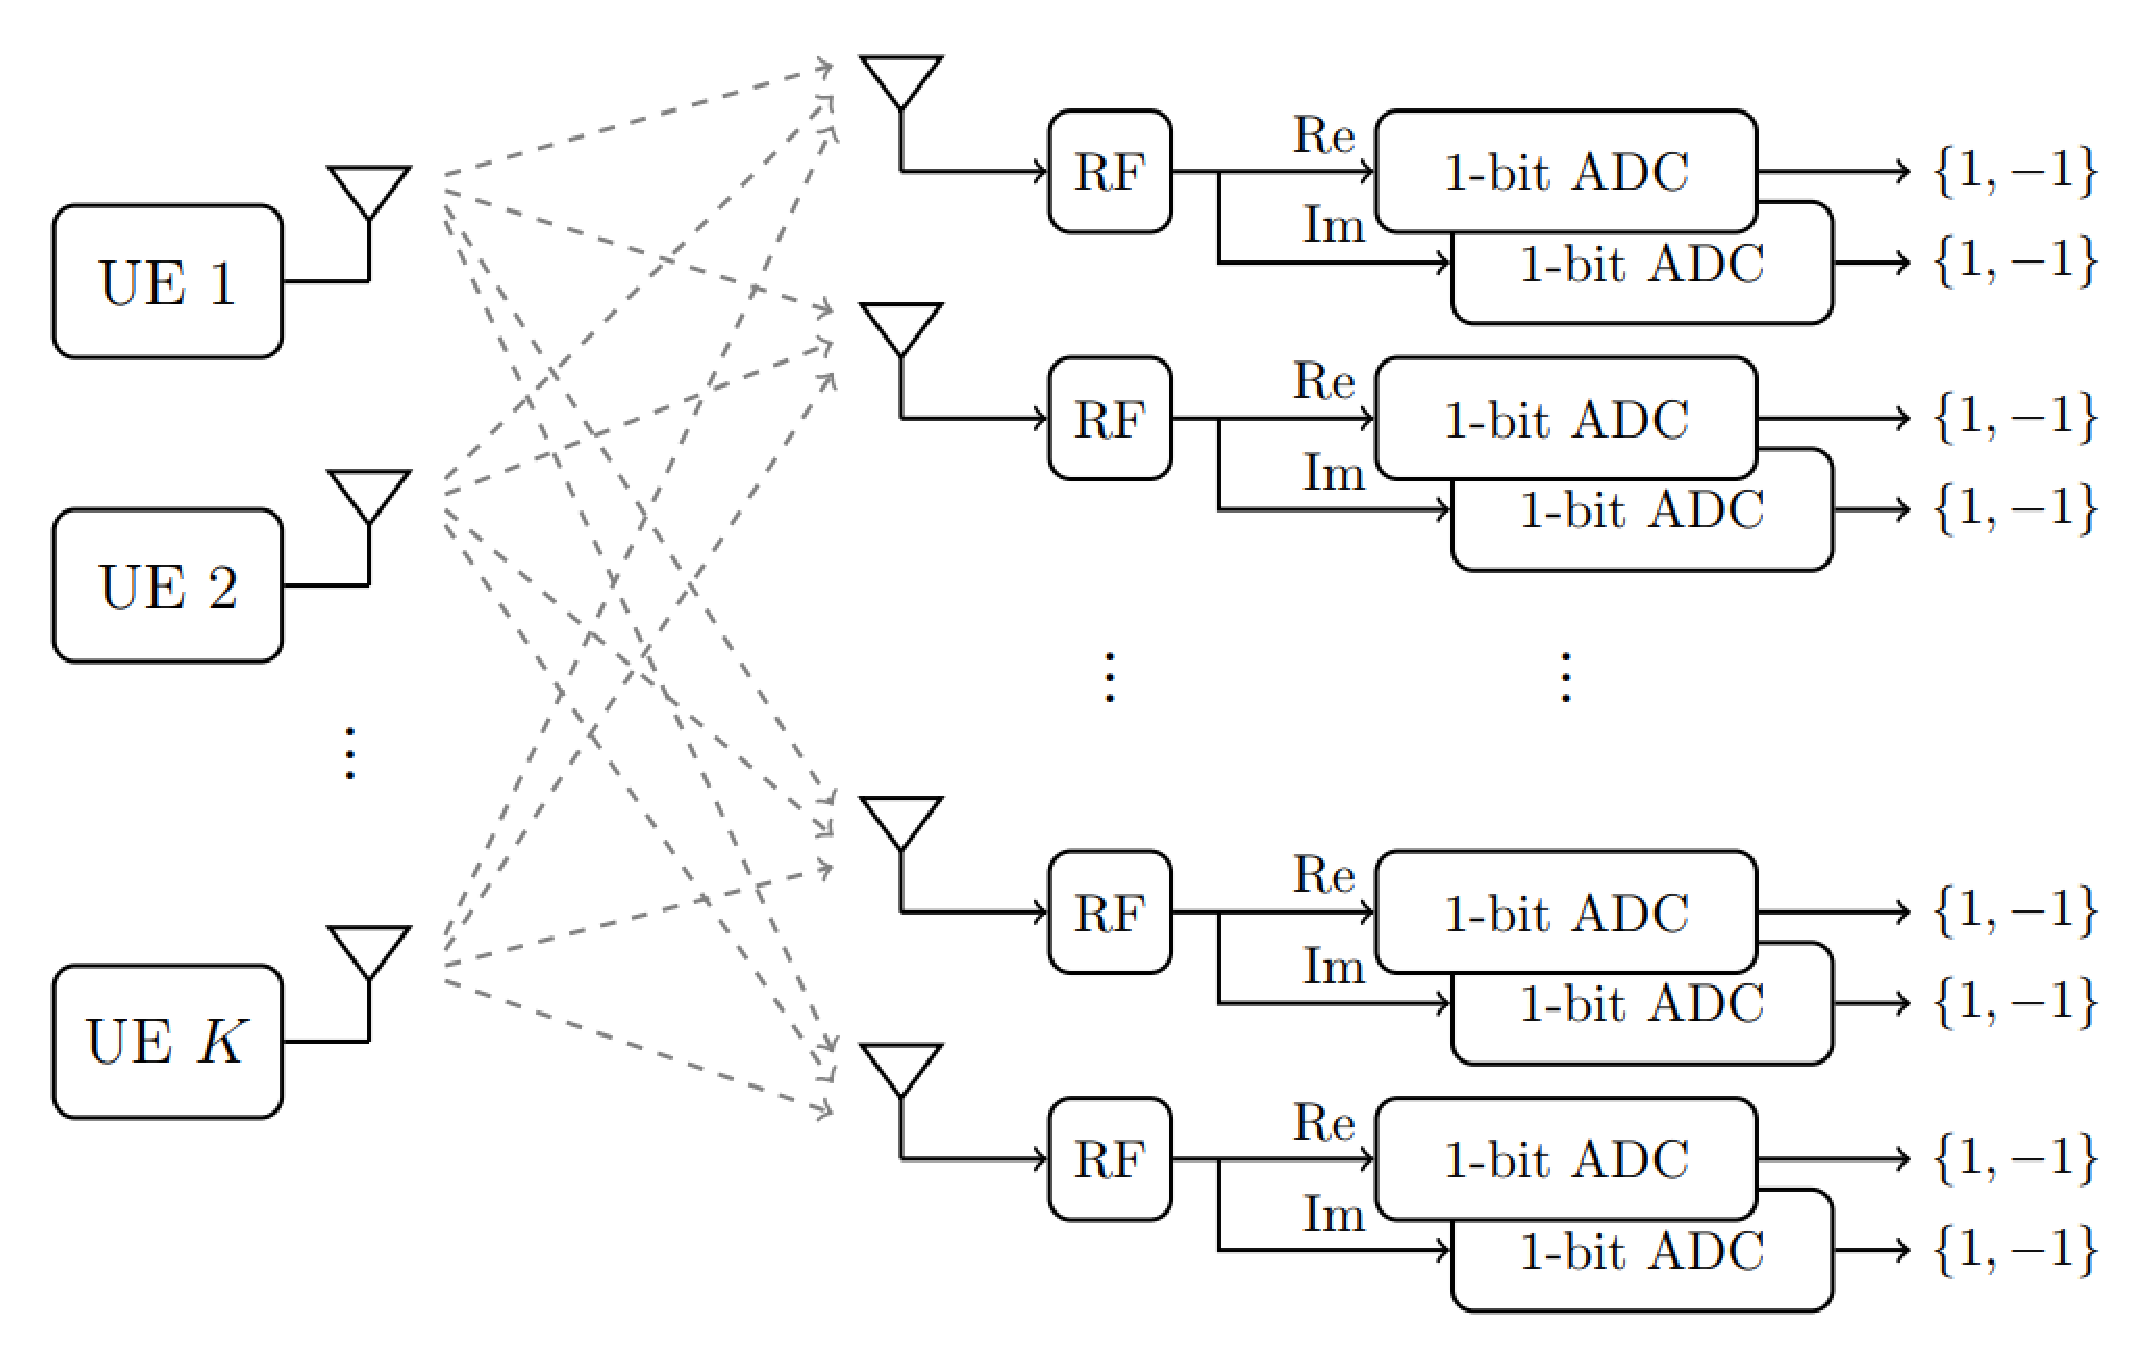
\includegraphics[scale=0.1]{Images/App_fig1.eps}
\end{figure}
\column{.33\textwidth}
\begin{figure}
	\centering
	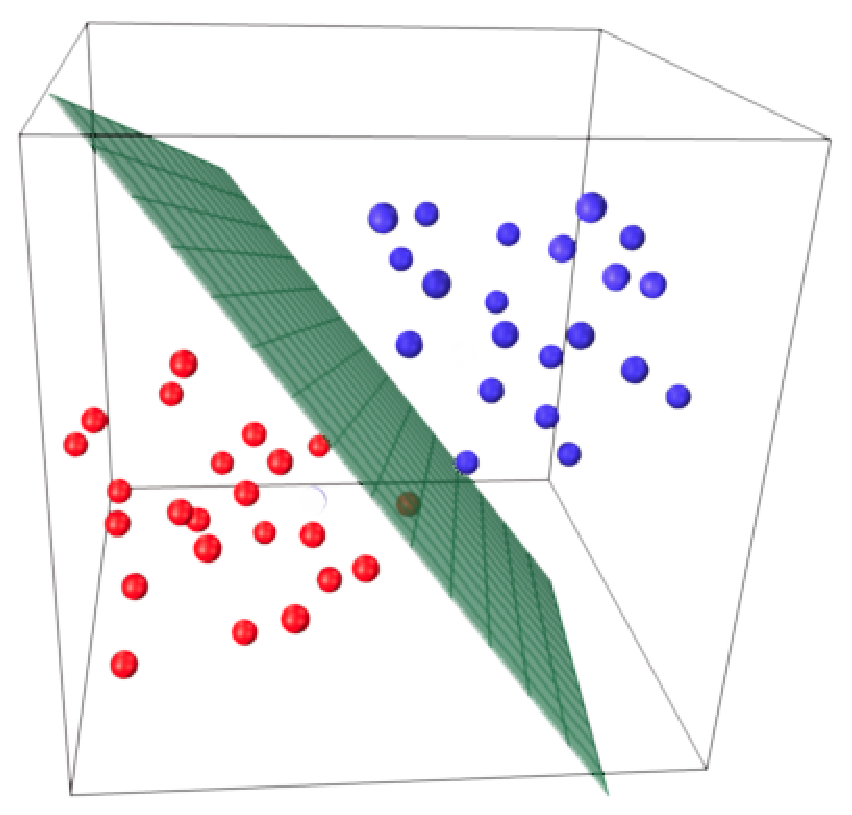
\includegraphics[scale=0.15]{Images/App_fig2.eps}
\end{figure}
\column{.33\textwidth}
\begin{figure}
	\centering
	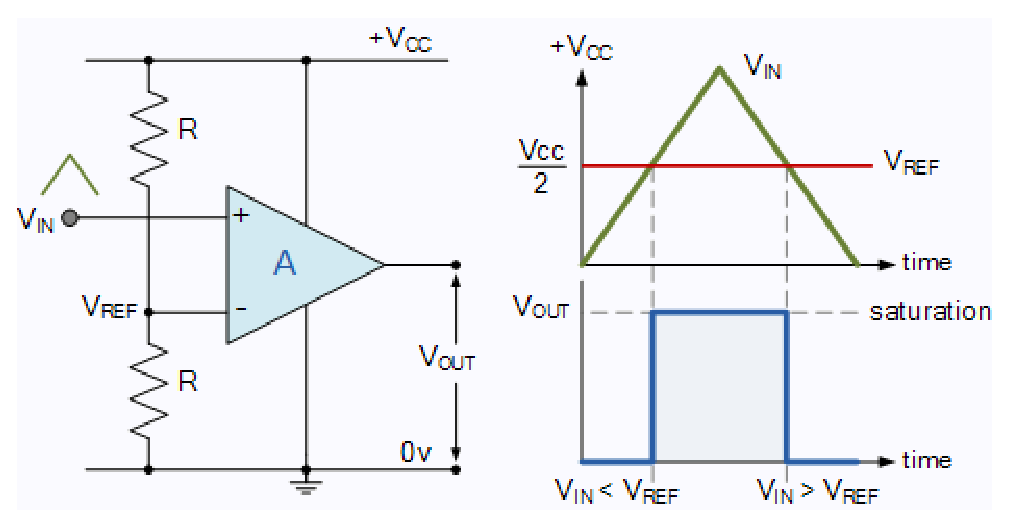
\includegraphics[scale=0.22]{Images/App_fig3.eps}
\end{figure}
\end{columns}

\begin{scriptsize}
\cite{risi2014massive,plan2013robust,baraniuk2017exponential}
\end{scriptsize}
\end{frame}
%%%%%%%%%%%%%%%%%%%%%%%%
%%%%%%%%%%%%%%%%%%%%%%%%
%%%%%%%%%%%%%%%%%%%%%%%%
%%%%%%%%%%%%%%%%%%%%%%%%
\section{سیگنال‌های دیکشنری تنک\hfill}
%%%%%%%%%%%%%%%%%%%%%%%%
\begin{frame}
\frametitle{سیگنال‌های دیکشنری تنک}
\begin{block}{}
\begin{center}
در بسیاری از کاربرد‌ها، سیگنال در یک دیکشنری تنک است.
\end{center}
\end{block}
\begin{columns}
\column{.5\textwidth}
\begin{figure}
\centering
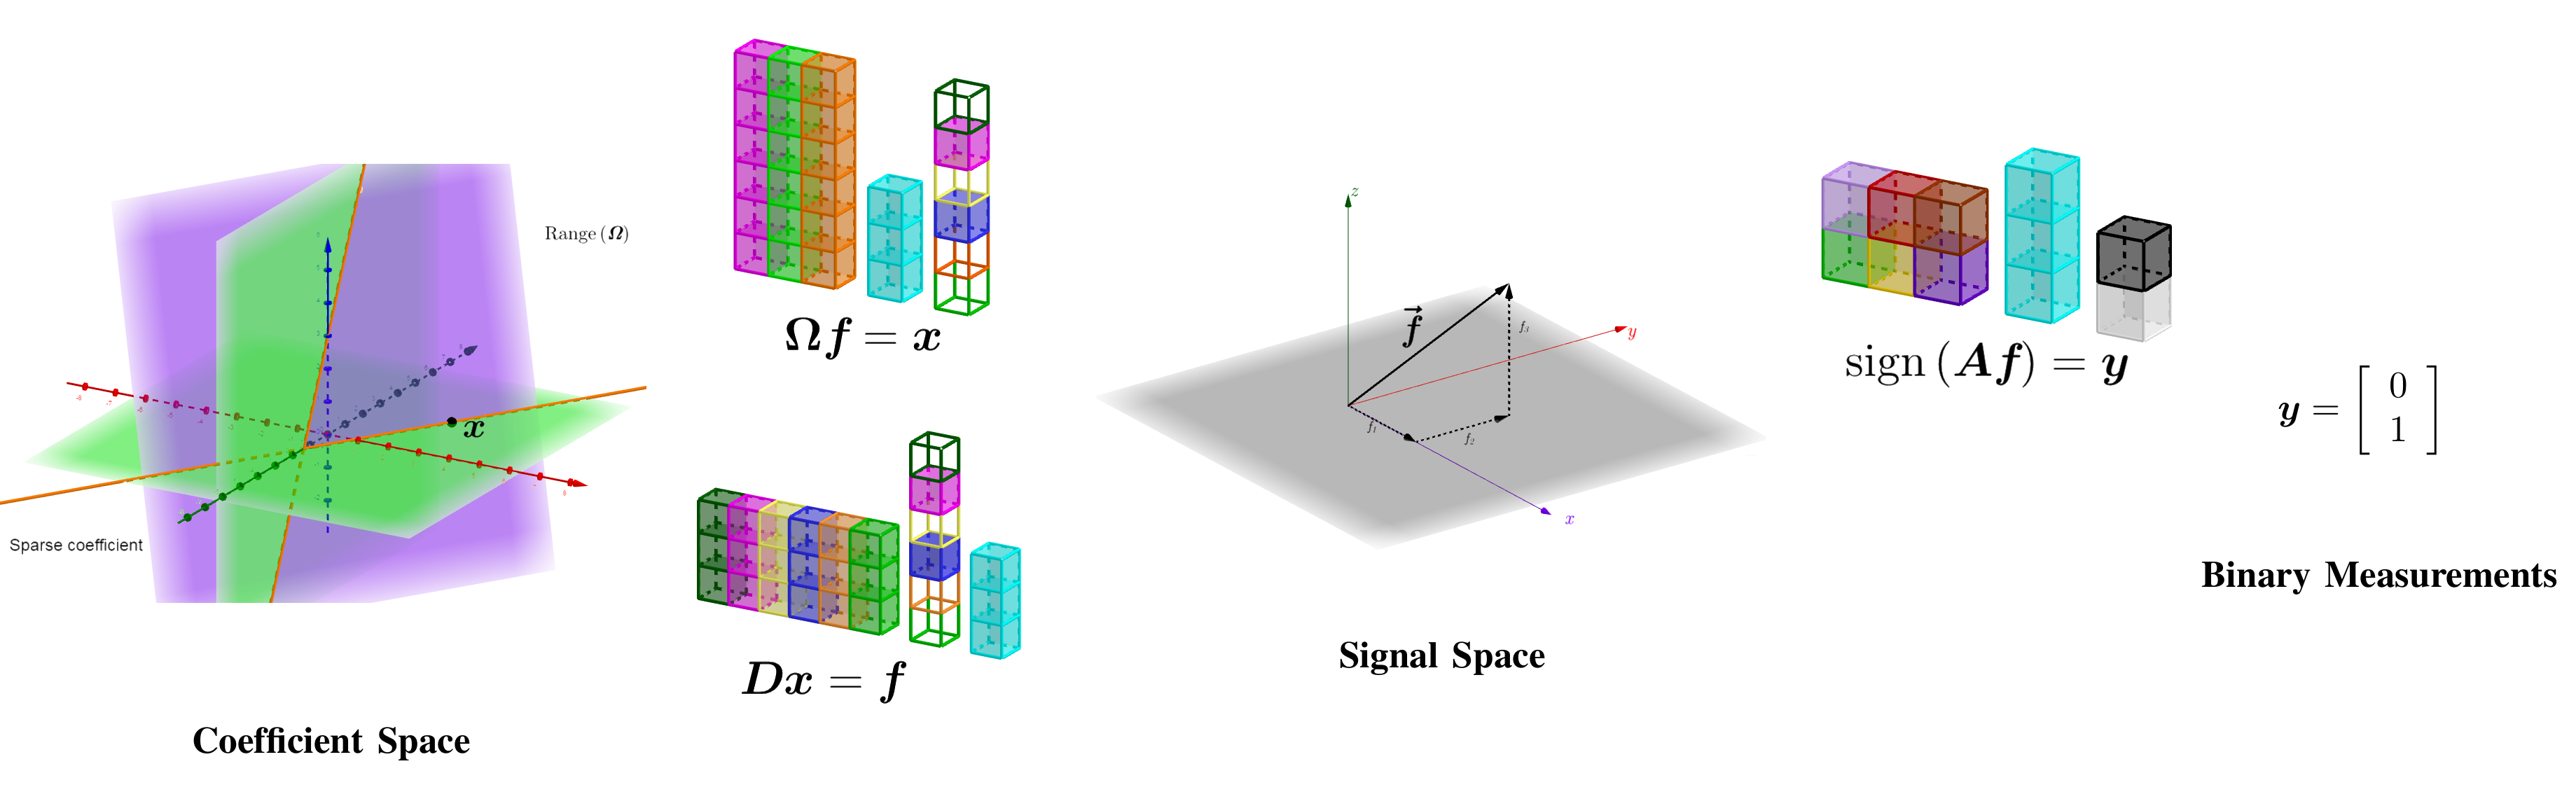
\includegraphics[scale=0.3]{Images/DS.png}
\end{figure}
\begin{scriptsize}
\cite{nam2013cosparse,Candes2011}
\end{scriptsize}
\column{.5\textwidth}
\begin{figure}
\centering
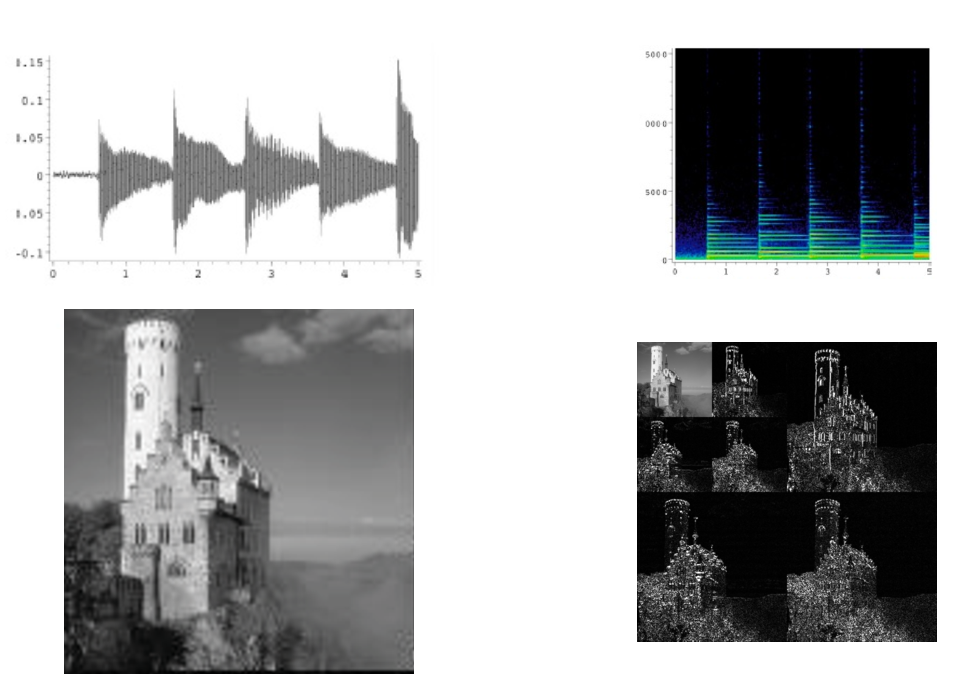
\includegraphics[scale=0.13]{Images/DS1.png}
\end{figure}
\end{columns}
\end{frame}

%%%%%%%%%%%%%%%%%%%%%%%%
\begin{frame}
\frametitle{سیگنال‌های دیکشنری تنک}
\begin{itemize}
\item{$\|\bm{x}\|_{0}\leq s$}
\end{itemize}
\begin{align}
\label{eq7}
\bm{f} = \bm{D}\bm{x}
\end{align}
\begin{columns}
\column{.33\textwidth}
\begin{center}
$\bm{x}\in \R^{N}$
\end{center}
\column{.33\textwidth}
\begin{center}
$\bm{D}\in \R^{n\times N}$
\end{center}
\column{.33\textwidth}
\begin{center}
$\bm{f}\in \R^{n}$
\end{center}
\end{columns}

\begin{columns}
\column{.5\textwidth}
\begin{block}{}
$\mu := \max_{1\leq i\neq j\leq N} \dfrac{| \langle d_{i},d_{j}\rangle|}{\norm{d_{i}}_{2}\norm{d_{j}}_{2}}$
\end{block}
\column{.5\textwidth}
\begin{itemize}
\item{
تنک-ترکیبی
\quad
$\bm{f}= \bm{D}\bm{x}$
}
\item{
تنک-تحلیلی
\quad
$\bm{D}^{\ast}\bm{f}$
}
\end{itemize}
\end{columns}
\end{frame}
%%%%%%%%%%%%%%%%%%%%%%%%
%%%%%%%%%%%%%%%%%%%%%%%%
%%%%%%%%%%%%%%%%%%%%%%%%
%%%%%%%%%%%%%%%%%%%%%%%%
\section{هندسه‌ی ابعاد بالا\hfill}
%%%%%%%%%%%%%%%%%%%%%%%%
\begin{frame}
\frametitle{هندسه‌ی ابعاد بالا}
\begin{columns}
\column{.5\textwidth}
\begin{figure}
\centering
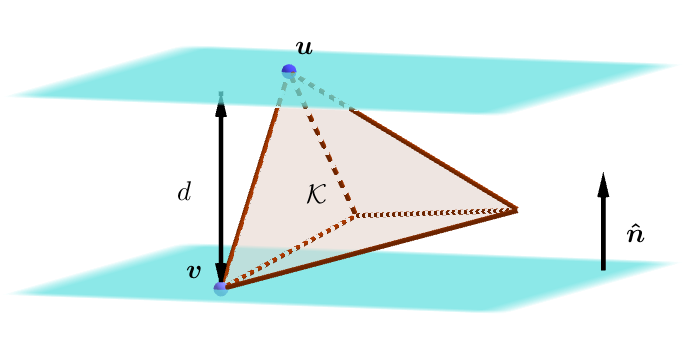
\includegraphics[scale=0.23]{Images/width.png}
\end{figure}
\begin{align*}
	d := \sup_{\bm{u},\bm{v}\in \mathcal{K}} \langle \hat{\bm{n}}, \bm{u}-\bm{v}  \rangle
\end{align*}
\column{.5\textwidth}
\begin{align*} 
\tilde{w}\left(\mathcal{K}\right) := \mathbb{E} \sup_{\bm{u},\bm{v}\in \mathcal{K}} \langle \hat{\bm{n}}, \bm{u}-\bm{v}  \rangle
\end{align*} 
با فرض بردار جهت گوسی:
\begin{align*}
w\left(\mathcal{K}\right) =  \mathbb{E} \norm{\bm{g}}_{2} \tilde{w}\left(\mathcal{K}\right)
\end{align*} 
\begin{itemize}
\item{$\mathcal{K}$
:مجموعه سیگنال‌های $s$-تنک
\begin{align*}
w\left(\mathcal{K}\right) = Cs \log\left(2n/s\right)
\end{align*}
}
\end{itemize}
\end{columns}
\end{frame}
%%%%%%%%%%%%%%%%%%%%%%%%
\begin{frame}
\frametitle{هندسه‌ی ابعاد بالا}
\framesubtitle{برش ابرصفحه تصادفی}
\begin{columns}
\column{.7\textwidth}
\begin{figure}
    \begin{overprint}
    \onslide<1>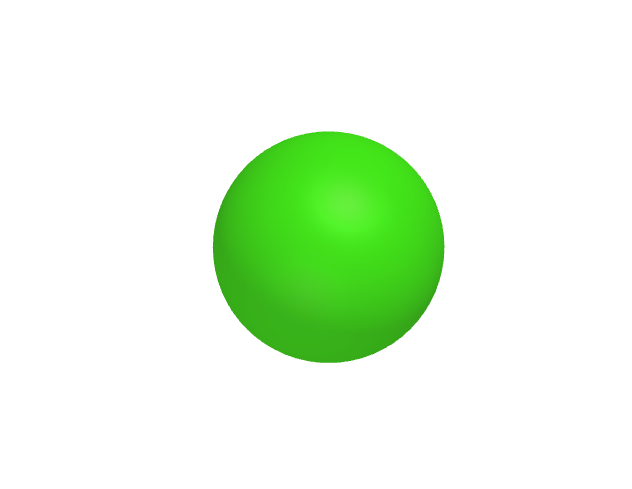
\includegraphics[scale=0.3]{Images/gif/1.png}
    \onslide<2>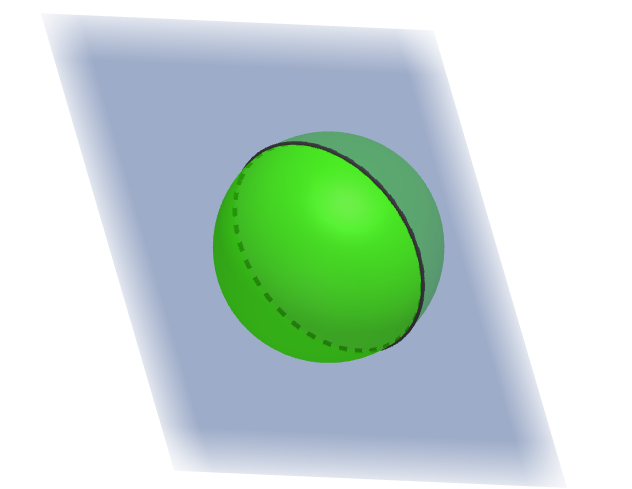
\includegraphics[scale=0.3]{Images/gif/2.png}
    \onslide<3>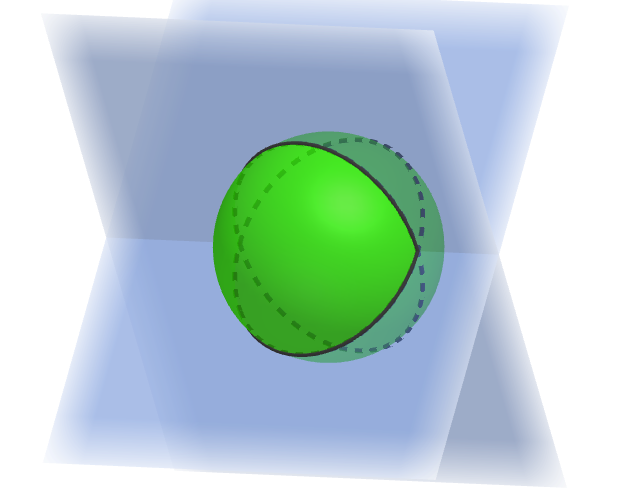
\includegraphics[scale=0.3]{Images/gif/3.png}
    \onslide<4>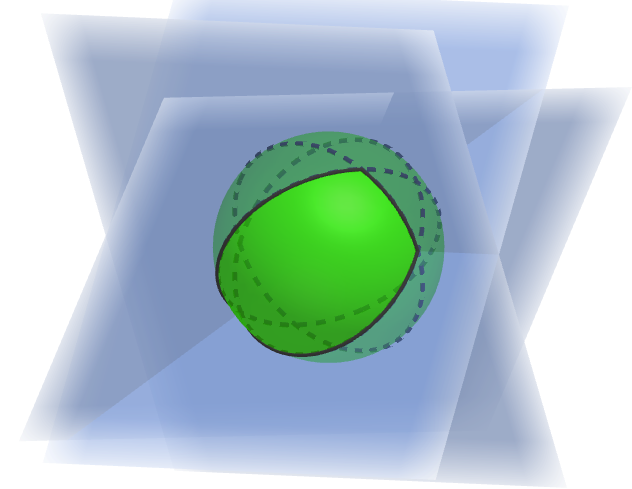
\includegraphics[scale=0.3]{Images/gif/4.png}
    \onslide<5>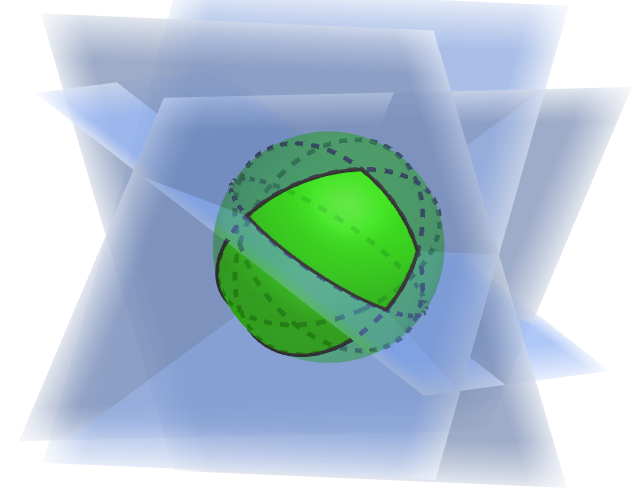
\includegraphics[scale=0.3]{Images/gif/5.png}
    \onslide<6-7>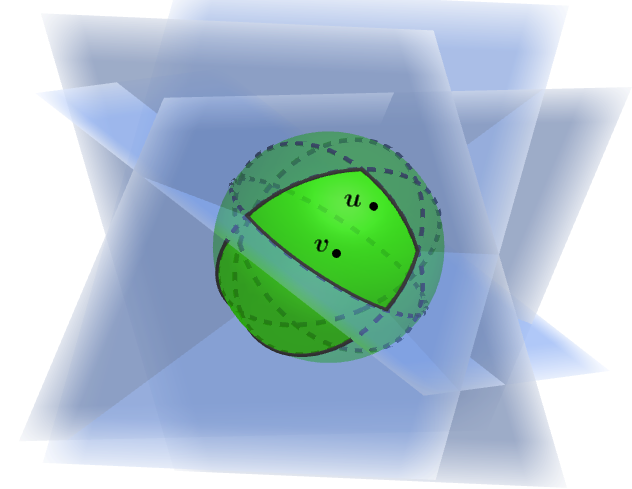
\includegraphics[scale=0.3]{Images/gif/6.png}
    \end{overprint}
\end{figure}
\column{.3\textwidth}
\only<1->{
\begin{align*}
y_{i} = \text{sign}(\langle\bm{a}_{i}, \bm{x}\rangle)
\end{align*}
}
\begin{itemize}
\only<1->{\item{$\bm{x}\in S^{n-1}$}}
\only<2->{\item{$y_{1}$}}
\only<3->{\item{$y_{2}$}}
\only<4->{\item{$y_{3}$}}
\only<5->{\item{$y_{4}$}}
\end{itemize}
\only<6>{
\begin{block}{}
\begin{center}
$\norm{\bm{u}-\bm{v}}_{2}\leq ?$\\
$ m=?$
\end{center}
\end{block}
}
\only<7>{
\begin{block}{}
\begin{center}
$\norm{\bm{u}-\bm{v}}_{2}\leq \delta $\\
$ m \geq C \delta^{-6} w\left(\mathcal{K}\right)^{2} $
\end{center}
\end{block}
}
\end{columns}
\end{frame}
%%%%%%%%%%%%%%%%%%%%%%%%
\begin{frame}
\frametitle{هندسه‌ی ابعاد بالا}
\framesubtitle{برش ابرصفحه تصادفی}
\begin{small}
\begin{theorem}[برش ابرصفحه تصادفی سیگنال دیکشنری تنک]
اگر
$ \mathcal{K}_{s}:= \left(\mathbf{D}^{\ast}\right)^{-1}\left(\Sigma_{s}^{N}\right)\cap S^{n-1} $
و
\begin{align*}
	m \geq C \epsilon^{-6} s \log\left(N/s\right)
\end{align*}
با احتمال
$1-\gamma\exp(-c\epsilon^{2}m)$
برای دو سیگنال 
$\bm{f},\bm{g}\in \mathcal{K}_{s}$
که در آن
\begin{align}
\text{sign}(\langle \bm{a}_i,\bm{f}\rangle)=\text{sign}(\langle \bm{a}_i,\bm{g}\rangle)
\end{align}
باشد، داریم
\begin{align}
\|\bm{f}-\bm{g}\|_{2}\leq \epsilon
\end{align}
\end{theorem}
\end{small}
\cite{Baraniuk2017}
\end{frame}
%%%%%%%%%%%%%%%%%%%%%%%%
%%%%%%%%%%%%%%%%%%%%%%%%
%%%%%%%%%%%%%%%%%%%%%%%%
%%%%%%%%%%%%%%%%%%%%%%%%
\section{الگوریتم پیشنهادی\hfill}
%%%%%%%%%%%%%%%%%%%%%%%%
\begin{frame}
\frametitle{مدل سیستم}
\begin{figure}
	\centering
	\includestandalone[scale=0.6]{Images/AdaptiveBD}
\end{figure}

\begin{block}{}
\begin{align*}
\label{eq:SSR}
 \bm{f}_{\varDelta}~=~\mathop{\arg\min}_{\bm{h}\in \R^{n} } \norm{\bm{D}^{*}\bm{h}}_{1}\quad \text{s.t.} \quad   \bm{y} =& \text{sign}\left(\bm{A}^{(i)}\bm{h}-\bm{\varphi}^{(i)} \right), \\
  & \norm{\bm{h}}_{2}\leq  r_t,
\end{align*}
\end{block}

\end{frame}
%%%%%%%%%%%%%%%%%%%%%%%%
\begin{frame}
\frametitle{آستانه‌ی ابعاد بالا}
\begin{algorithm}[H]
	\caption{$ \Phi $: مولد آستانه در ابعاد بالا}
	\label{alg:HDTG}
	\begin{algorithmic}[1]
		\renewcommand{\algorithmicrequire}{\textbf{ورودی:}}
		\renewcommand{\algorithmicensure}{\textbf{خروجی:}}
		\REQUIRE ماتریس اندازه‌گیری $ \bm{A} $, تعداد نمونه‌ها $ b $, واریانس لغزش‌ها $ \sigma^{2} $, سیگنال تخمینی $ \hat{\bm{f}} $.
		\ENSURE بردار آستانه در ابعاد بالا $\bm{\varphi}\in \R^{b}$.
		\STATE $ \bm{\tau}\sim N(0,\sigma^{2}\bm{I}_{b} ) $
		\STATE  $ \bm{\varphi}=\bm{A}\hat{\bm{f}}+\bm{\tau} $
	\end{algorithmic} 
\end{algorithm}
\end{frame}
%%%%%%%%%%%%%%%%%%%%%%%%
\begin{frame}
\frametitle{آستانه‌ی ابعاد بالا}
\begin{columns}
\column{.3\textwidth}
\begin{scriptsize}
\begin{align*}
\bm{y}^{(t)}=& \text{sign}\left( \bm{A}^{(t)}\bm{f}- \bm{\varphi}^{(t)}\right) \\
=& \text{sign}\left( \bm{A}^{(t)}\bm{f}- \bm{A}^{(t)}\bm{f}_{t-1}-\bm{\tau}^{(t)}\right) \\
=&\text{sign}\left( \bm{A}^{(t)}\left(\bm{f}-\bm{f}_{t-1}\right)-\bm{\tau}^{(t)}\right)
\end{align*}
\end{scriptsize}
\column{.7\textwidth}
\begin{figure}
    \begin{overprint}
    \onslide<1>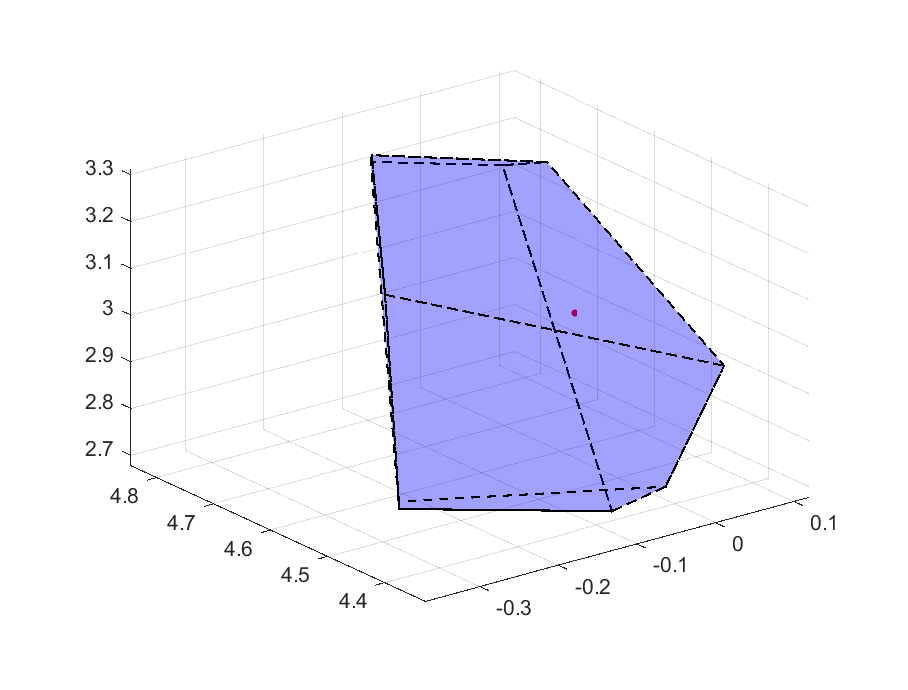
\includegraphics[scale=0.5]{Images/polyhdr1.eps}
    \onslide<2>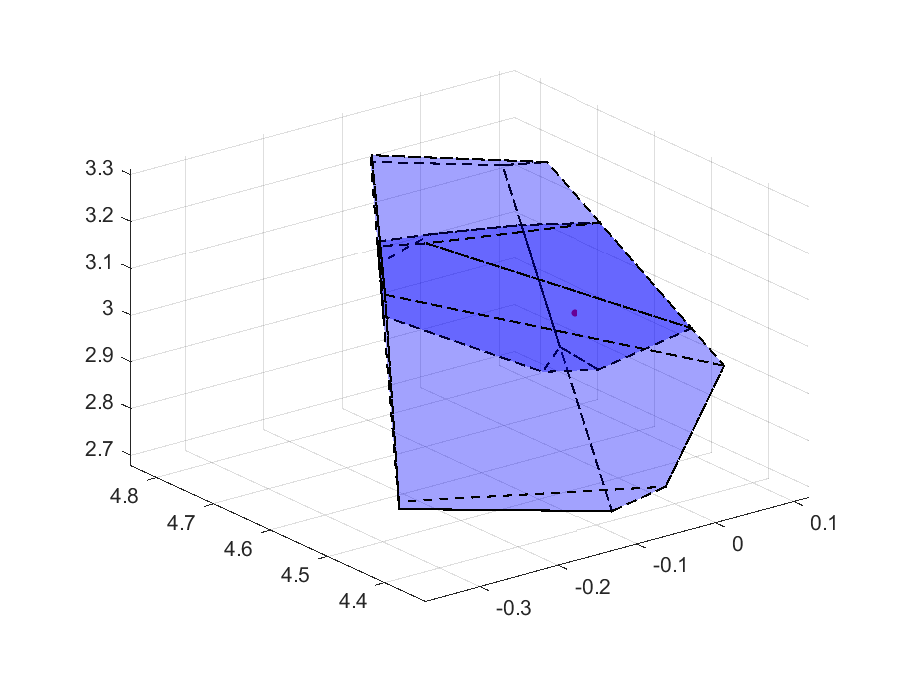
\includegraphics[scale=0.5]{Images/polyhdr2.eps}
    \onslide<3>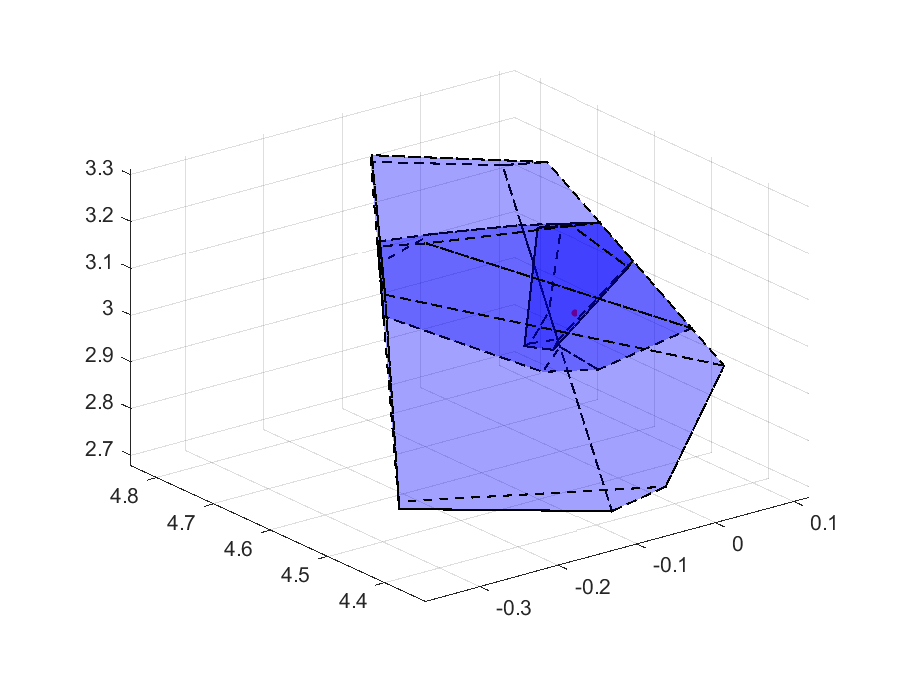
\includegraphics[scale=0.5]{Images/polyhdr3.eps}
    \end{overprint}
\end{figure}
\end{columns}
\end{frame}
%%%%%%%%%%%%%%%%%%%%%%%%
\begin{frame}
\begin{block}{}
\begin{center}
تفاوت آستانه‌ی تصادفی معمولی با آستانه‌ی تصادفی ابعاد بالا
\end{center}
\end{block}
\begin{columns}
\column{.5\textwidth}
\begin{align*}
 \bm{y}^{\left(i\right)} = \text{sign}\left(\bm{A}^{(i)}\bm{f}-\bm{\tau}^{\left(i\right)}\right)
\end{align*}
\begin{figure}
\centering
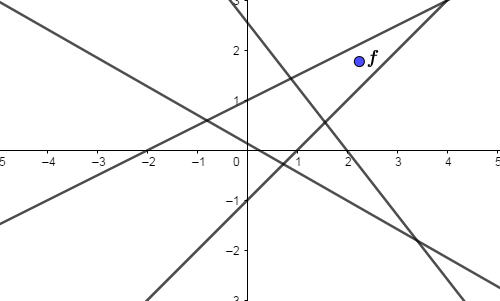
\includegraphics[scale=0.3]{Images/HDT1.png}
\end{figure}
\column{.5\textwidth}
\begin{align*}
 \bm{y}^{\left(i\right)} = \text{sign}\left(\bm{A}^{(i)}\bm{f}-\bm{\varphi}^{\left(i\right)}\right)
\end{align*}
\begin{figure}
\centering
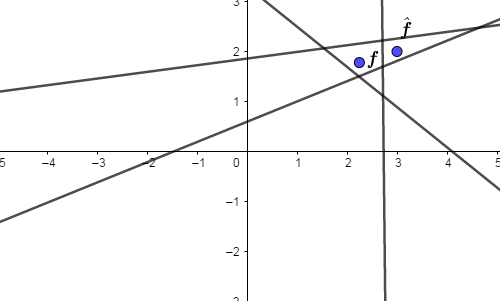
\includegraphics[scale=0.3]{Images/HDT2.png}
\end{figure}
\end{columns}
\end{frame}
%%%%%%%%%%%%%%%%%%%%%%%%
\begin{frame}
\frametitle{نمونه‌برداری وفقی}
\begin{algorithm}[H]
	\caption{$ \mathcal{Q} $: نمونه‌برداری وفقی}
	\label{alg:AQ}
	\begin{algorithmic}[1]
		\renewcommand{\algorithmicrequire}{\textbf{ورودی:}}
		\renewcommand{\algorithmicensure}{\textbf{خروجی:}}
		\REQUIRE دیکشنری $ \bm{D}\in\R^{n\times N} $, ماتریس نمونه‌برداری $ \bm{A}\in\R^{m\times n} $, مشاهدات خطی $ \bm{Af}\in \R^{m} $, تخمین نورم $ \norm{\bm{f}}_{2}\leq r $, تعداد بلوک‌ها $ L $.
		\ENSURE  نمونه‌های کوانتیزه $ \bm{y} \in \lbrace\pm 1\rbrace^{m} $, آستانه‌ها در ابعاد بالا $ \bm{\varphi} \in \R^{m} $
		\\ \textit{مقدار‌دهی اولیه} : $ \bm{f}_{0}\leftarrow \bm{0} $, $ b = \lfloor\frac{m}{L}\rfloor $, $ \bm{A}^{(i)}\in \R^{b\times m}  $
		\begin{latin}
		\FOR {$i = 1,\cdots,L$}
		\STATE $r_{t}=2^{1-t}r$
		\STATE $\bm{\varphi}^{\left(i\right)}\leftarrow \Phi(\bm{A}^{(i)},b,2^{1-t}r,\bm{f}_{i-1}) $
		\STATE $ \bm{y}^{\left(i\right)} = \text{sign}\left(\bm{A}^{(i)}\bm{f}-\bm{\varphi}^{\left(i\right)}\right)$
		\STATE $ \bm{f}_{i} = \bm{f}_{i-1} + \varDelta\left(\bm{D},\bm{A}^{(i)},\bm{y}^{\left(i\right)},\bm{\varphi}^{\left(i\right)},\bm{r}_{t}\right) $
		\ENDFOR
		\end{latin}
	\end{algorithmic} 
\end{algorithm}
\end{frame}
%%%%%%%%%%%%%%%%%%%%%%%%
\begin{frame}
\frametitle{بازیابی وفقی}
\begin{algorithm}[H]
	\caption{$ \mathcal{R} $: بازیابی وفقی}
	\label{alg:AR}
	\begin{algorithmic}[1]
		\renewcommand{\algorithmicrequire}{\textbf{ورودی:}}
		\renewcommand{\algorithmicensure}{\textbf{خروجی:}}
		\REQUIRE دیکشنری $ \bm{D}\in\R^{n\times N} $, ماتریس نمونه‌برداری $ \bm{A}\in\R^{m\times n} $, نمونه‌های کوانتیزه $ \bm{y} \in \lbrace\pm 1\rbrace^{m} $, آستانه‌ها در ابعاد بالا $ \bm{\varphi}\in\R^{m} $, تخمین نورم $ \norm{\bm{f}}_{2}\leq r $, تعداد بلوک‌ها $ L $.
		\ENSURE  تخمین سیگنال $ \hat{\bm{f}}\in \R^{n} $.
		\\ \textit{مقداردهی اولیه} :  $ b = \lfloor\frac{m}{L}\rfloor $, $ \bm{A}^{(i)}\in \R^{b\times m}$, $ \bm{y}^{\left(i\right)} \lbrace\pm 1\rbrace^{b}$, $\bm{\varphi}^{\left(i\right)}\in \R^{b} $
		\begin{latin}
		\FOR {$i = 1,\cdots,L$}
		\STATE $ \bm{f}_{i} =\bm{f}_{i-1}+ \varDelta\left(\bm{D},\bm{A}^{(i)},\bm{y}^{\left(i\right)},\bm{\varphi}^{\left(i\right)},\bm{r}_{t}\right) $ 
		\ENDFOR
		\end{latin}
	\end{algorithmic} 
\end{algorithm}
\end{frame}
%%%%%%%%%%%%%%%%%%%%%%%%
\begin{frame}
\frametitle{کران خطا}
\begin{theorem}
با فرض دریافت
\begin{align}
 m \geq C(r/\sigma+\sigma / r)^{6}(r^{2}/\sigma^2+1)(\epsilon+2)^{-6}s \log (N/s) 
\end{align} 
نمونه با استفاده از الگوریتم نمونه‌برداری وفقی
(الگوریتم\ref{alg:AQ})
با احتمال 
\begin{align}
 1-\gamma \exp{(-c^{\prime}m (\epsilon+2)^{2} r^2\sigma^2/ (r^2+\sigma^2)^2)} 
\end{align}
خروجی الگوریتم بازیابی وفقی
(الگوریتم\ref{alg:AR}) 
در شرط  
\begin{align}
\|\bm{f}-\hat{\bm{f}}\|_{2}\leq \epsilon r2^{1-L},
\end{align}
صدق می‌کند.
\end{theorem}

\end{frame}
%%%%%%%%%%%%%%%%%%%%%%%%
\begin{frame}
\frametitle{تعبیر شهودی}
\begin{itemize}
\item{تصویر بر نیم‌کره}
\end{itemize}
\begin{figure}
    \begin{overprint}
    \onslide<1>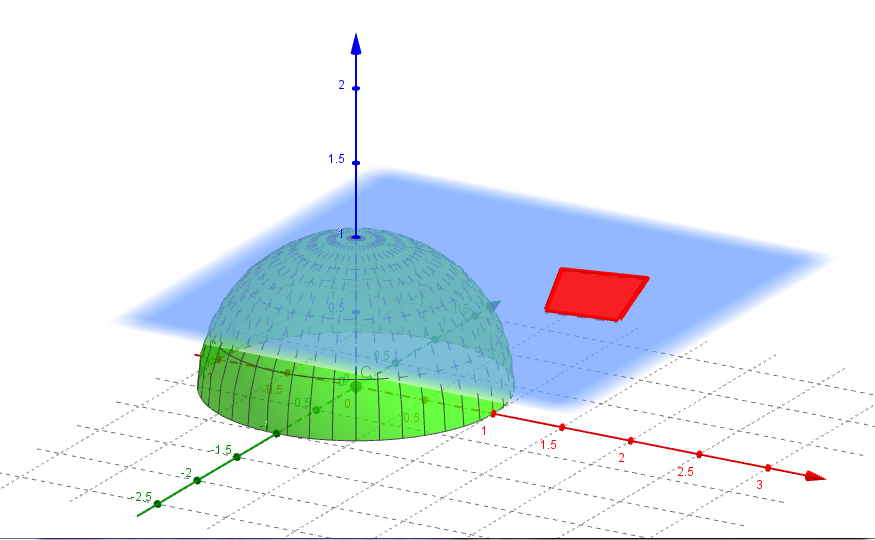
\includegraphics[scale=0.4]{Images/HPfig1.png}
    \onslide<2>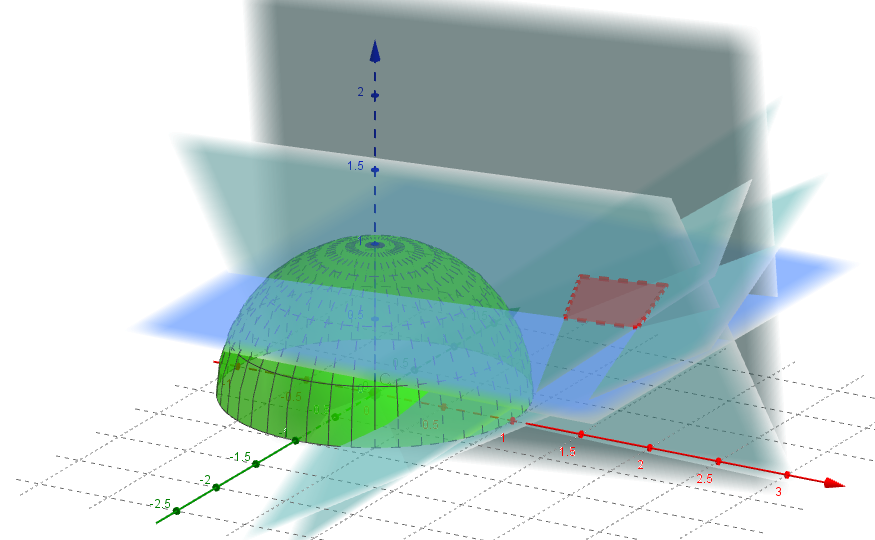
\includegraphics[scale=0.4]{Images/HPfig2.png}
    \onslide<3>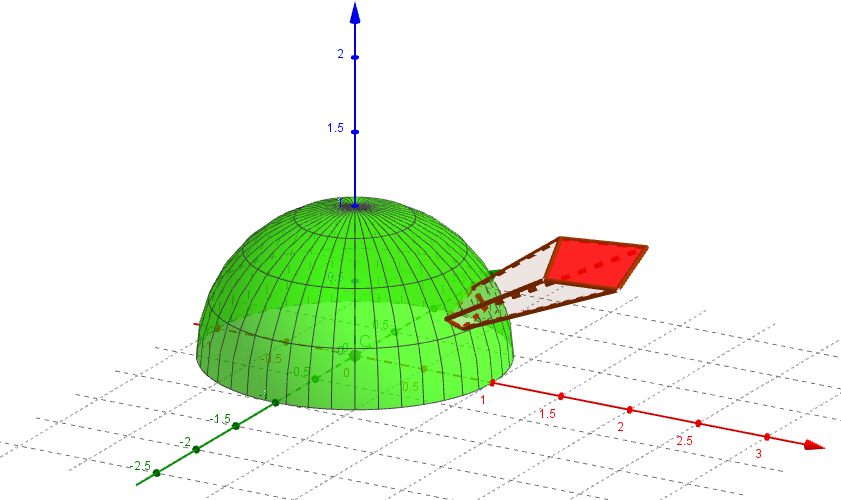
\includegraphics[scale=0.4]{Images/HPfig3.png}
    \end{overprint}
\end{figure}
\end{frame}
%%%%%%%%%%%%%%%%%%%%%%%%
\begin{frame}
\frametitle{تعبیر شهودی}
\begin{itemize}
\item{تصویر بر نیم‌کره}
\end{itemize}
\begin{columns}
\column{.5\textwidth}
\begin{figure}
	\centering
	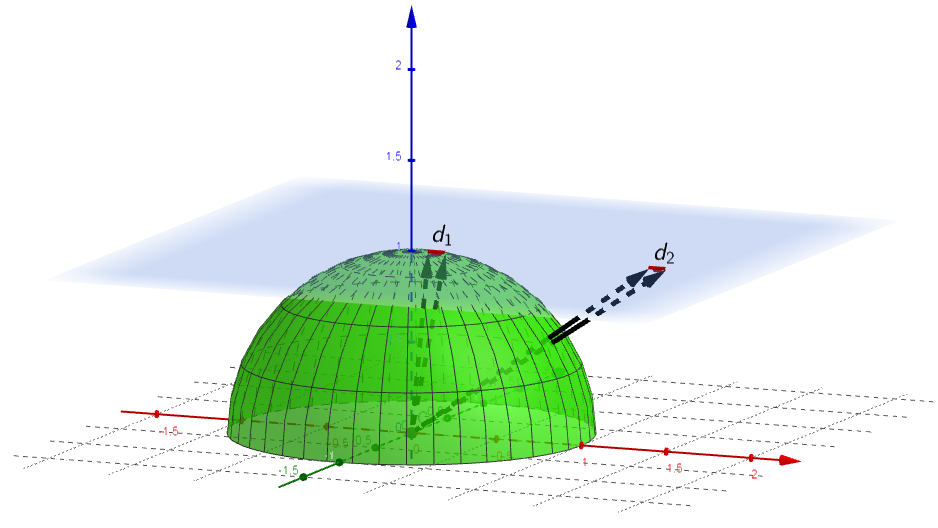
\includegraphics[scale=0.15]{Images/HP1.png}
\end{figure}
\column{.5\textwidth}
\begin{figure}
	\centering
	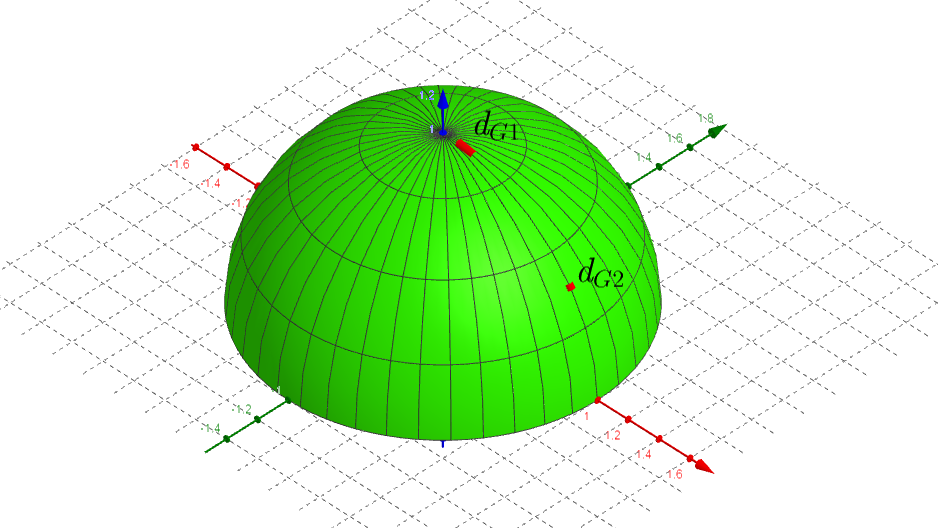
\includegraphics[scale=0.15]{Images/HP2.png}
\end{figure}
\end{columns}

\begin{align}
P_{H}(\tilde{\bm{f}}) = \dfrac{\tilde{\bm{f}}}{\|\tilde{\bm{f}}\|_{2}}\quad \quad \tilde{\bm{f}}:= [\bm{f}^{T}~|~\sigma]^{T}\in \R^{N+1}
\end{align}

\end{frame}
%%%%%%%%%%%%%%%%%%%%%%%%
%%%%%%%%%%%%%%%%%%%%%%%%
%%%%%%%%%%%%%%%%%%%%%%%%
%%%%%%%%%%%%%%%%%%%%%%%%

\section{نتایج شبیه‌سازی\hfill}

\begin{frame}
\frametitle{نتایج شبیه‌سازی}
\begin{align*}
N= 1000, \quad n= 50, \quad s= 10, \quad L=10
\end{align*}
\begin{figure}
	\centering
	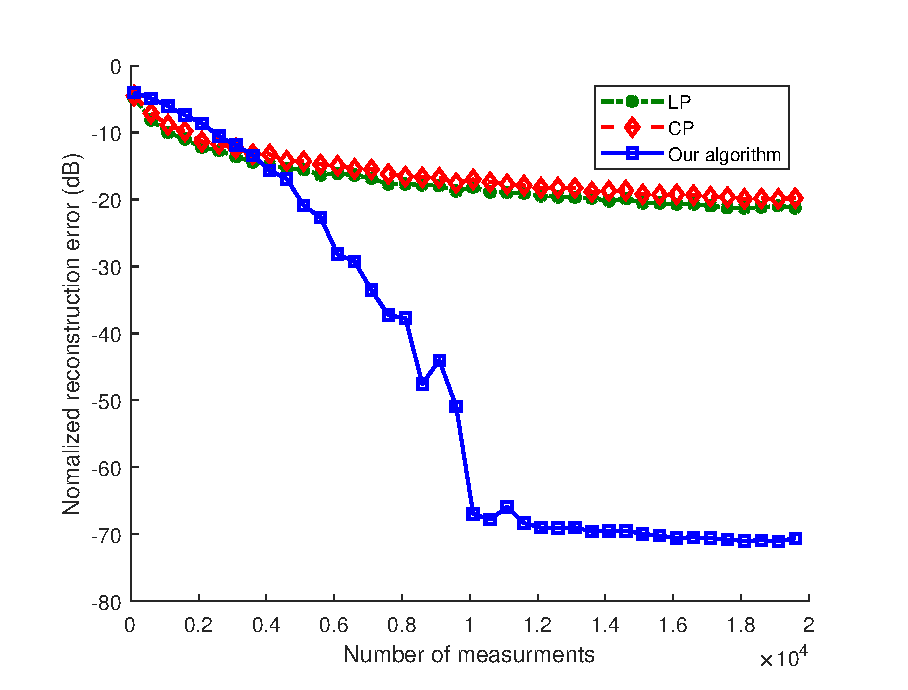
\includegraphics[scale=0.45]{Images/simfig1.eps}
\end{figure}
\end{frame}
%%%%%%%%%%%%%%%%%%%%%%%%
\begin{frame}
\frametitle{نتایج شبیه‌سازی}
\begin{figure}
\centering
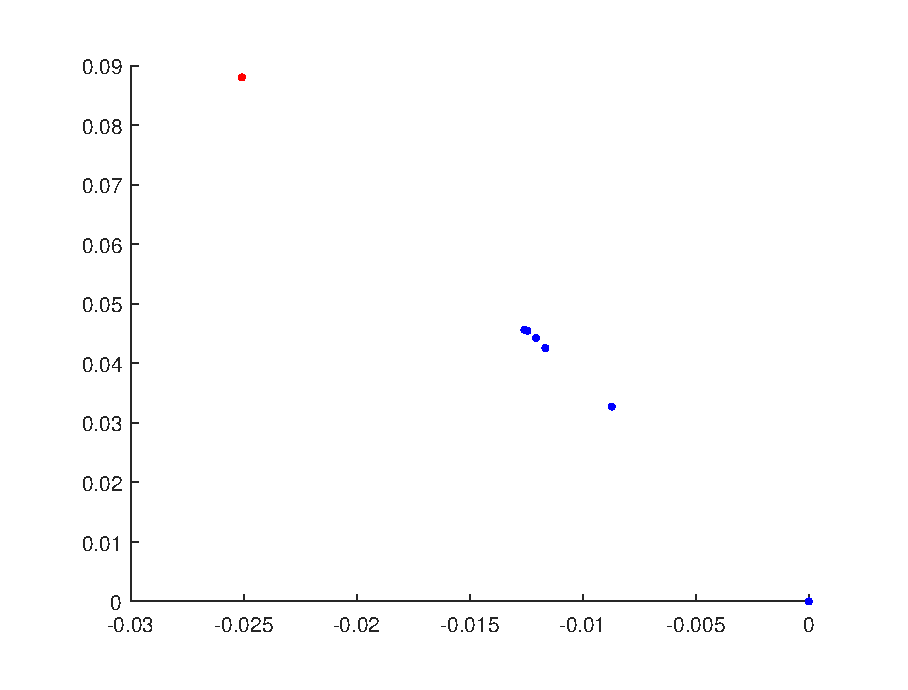
\includegraphics[scale=0.5]{Images/eer.eps}
\end{figure}
\end{frame}
%%%%%%%%%%%%%%%%%%%%%%%%
\begin{frame}
\frametitle{نتایج شبیه‌سازی}
\begin{align*}
N= 1000, \quad n= 50, \quad s= 10,20,30,40,50 \quad L=10
\end{align*}
\begin{figure}
	\centering
	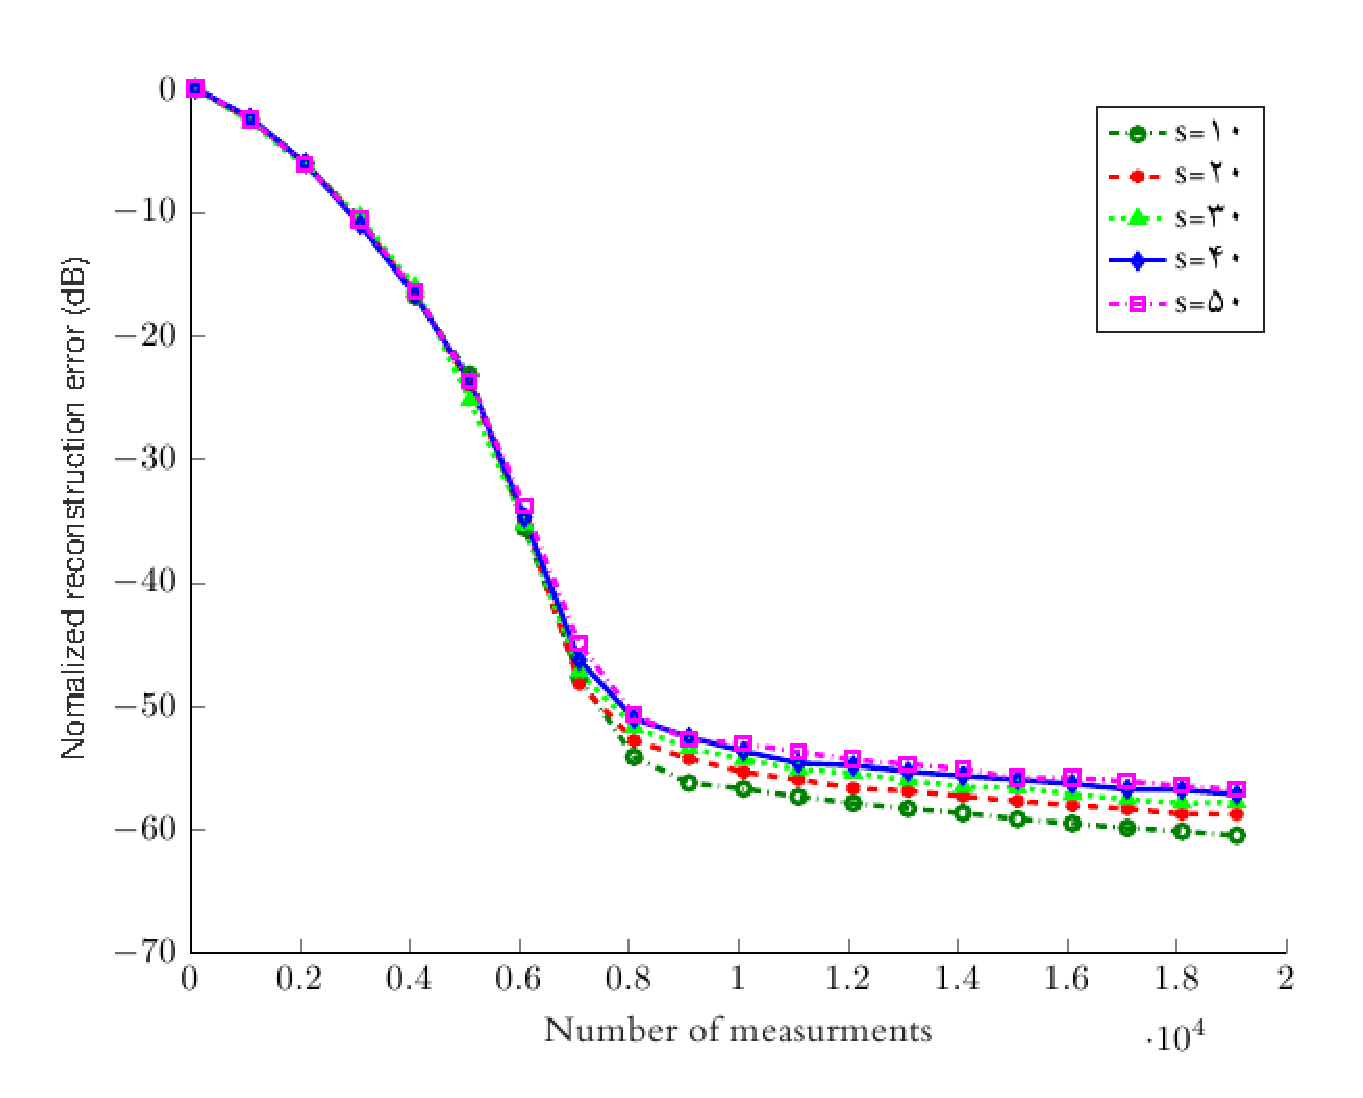
\includegraphics[scale=0.25]{Images/simfig2.eps}
\end{figure}
\end{frame}
%%%%%%%%%%%%%%%%%%%%%%%%
%%%%%%%%%%%%%%%%%%%%%%%%
%%%%%%%%%%%%%%%%%%%%%%%%
%%%%%%%%%%%%%%%%%%%%%%%%
